\documentclass{beamer}
\usepackage{beamerthemesplit}
\usepackage{color}
\usepackage{amsfonts}
\usepackage{wrapfig}
\usepackage{multicol}
\setlength{\columnsep}{0cm}

\definecolor{Blue}{RGB}{51,51,153}
\mode<presentation>
{
\usetheme[]{Darmstadt}
}
\title{Marchiatura digitale di sequenze video stereoscopiche a disparità coerente}
\author{Benedetta Barbetti\\ 
		Michaela Servi}
\institute{Universit\`{a} degli studi di Firenze}
\date{10 Dicembre 2015}


\begin{document}

\begin{frame}
\titlepage
\end{frame}

\begin{section}{Introduzione}
\subsection{Proteine RNA-binding}
\begin{frame}
\frametitle{Proteine RNA-binding}
\begin{columns}[T]
\begin{column}[T]{6cm}
\begin{itemize}
\item L'RNA interagisce con le proteine per portare a termine molti dei suoi compiti
\item Con il termine \textbf{RNA-binding protein} si intende una proteina in grado di instaurare legami con l'RNA
\end{itemize}
\end{column}
\begin{column}[T]{4cm}
\begin{figure}
  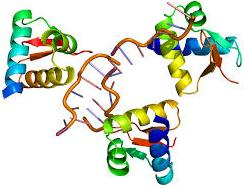
\includegraphics[width=1\textwidth]{./img/rna_binding}
  
  \label{fig:rna_binding}
\end{figure}
\end{column}
\end{columns}
\begin{itemize}
\item Per capire i meccanismi di questa interazione sono state proposte diverse tecniche che si differenziano sia per algoritmo implementato sia per feature in input 
\end{itemize}
\end{frame}

\subsection{Stato dell'arte}
\begin{frame}
\frametitle{RNA-binding sites prediction methods}
\scalebox{0.6}{
\begin{tabular}{llll}
\hline \hline
Group & Algorithm & Input Info & Category\\ \hline
Jeong et at., 2004 & Neural Network & Binary vector + predicted secondary structure & Single sequence \\
Jeong and Miyano, 2006 &  & PSSM  & Multiple sequence\\
Terribilini et at., 2006 & Naive Bayes &  Binary vector & 	
					Single sequence \\
					& SVM(RBF) & PSSM & Multiple sequence\\	
Wang and Brown, 2006 & SVM(RBF) & Hydrophobicity & Single sequence \\
Kumar et at., 2007 & SVM & Binary vector & Single sequence \\ 
					&  & PSSM & Multiple sequence\\
\hline 
\end{tabular}
}
\end{frame}

\subsection{Kumar et al., 2007}
\begin{frame}
\frametitle{Kumar et al., 2007}
\begin{itemize}
\item Classificatore basato su sequenze singole e multiple
\item Dataset di \textbf{86} proteine (Jeong et al., 2006)
\item Ogni amino acido \`{e} stato codificato come un \textbf{vettore binario} o un vettore \textbf{PSSM} ottenuto con una ricerca PSI-BLAST sul NCBI nonredundant database
\item Come input alla \textbf{SVM} \`{e} stato utilizzata una sliding window
\item La predizione migliore \`{e} stata ottenuta utilizzando l'encoding PSSM, che ha prodotto un'accuratezza di \textbf{0.81} e un MCC di 0.45 
\end{itemize}
\end{frame}
\end{section}

\begin{section}{Metodo di Kumar et al., 2007}
\subsection{Dataset}
\begin{frame}
\frametitle{RNA\_86}
\begin{itemize}
\item 86 catene proteiche RNA-binding estratte dalle strutture dei complessi di RNA-proteina
\item Le strutture sono state ottenute dalla Protein Data Bank
\item La similarit\`{a} tra coppie di catene \`{e} minore del 70\%
\item Ogni catena proteica ha almeno 4 RNA-interacting residui
\item \textbf{20071} residui, \textbf{4568} dei quali sono RNA-interacting residui
\end{itemize}
\end{frame}

\subsection{Support Vector Machines}
\begin{frame}
\frametitle{Support Vector Machines}
\begin{itemize}
\item Per la classificazione dei RNA-interacting residui sono state utilizzate le \textbf{SVMs}, implementate utilizzando la libreria \texttt{sklearn}
\item Applicate con successo a numerosi problemi di regressione e classificazione di pattern, tra cui problemi di bioinformatica
\end{itemize}
\end{frame}

\begin{frame}
\frametitle{Definizione}
Dati $ \boldsymbol{x_{i}} \in R^{p}, i=1,...,n,$ in 2 classi, e un vettore $ \boldsymbol{y} \in R^{p}$ tale che $y \in \{-1,1\}$, SVC risolve il seguente problema:\newline
\begin{columns}
\begin{column}{6cm}
\begin{center}
$\displaystyle\min_{\omega, b, \zeta} \ \frac{1}{2} \ \omega^{T}\omega + \mathrm{C} \sum_{i=1,n} \zeta_{i}$\newline
subject to $y_{i}(\omega^{T}\phi(x_{i}) + b) \ge 1 - \zeta_{i}$\newline
$\zeta_{i} \ge 0, i = 1,...,n$
\end{center}
\end{column}
\begin{column}{4cm}
\begin{figure}
\centering
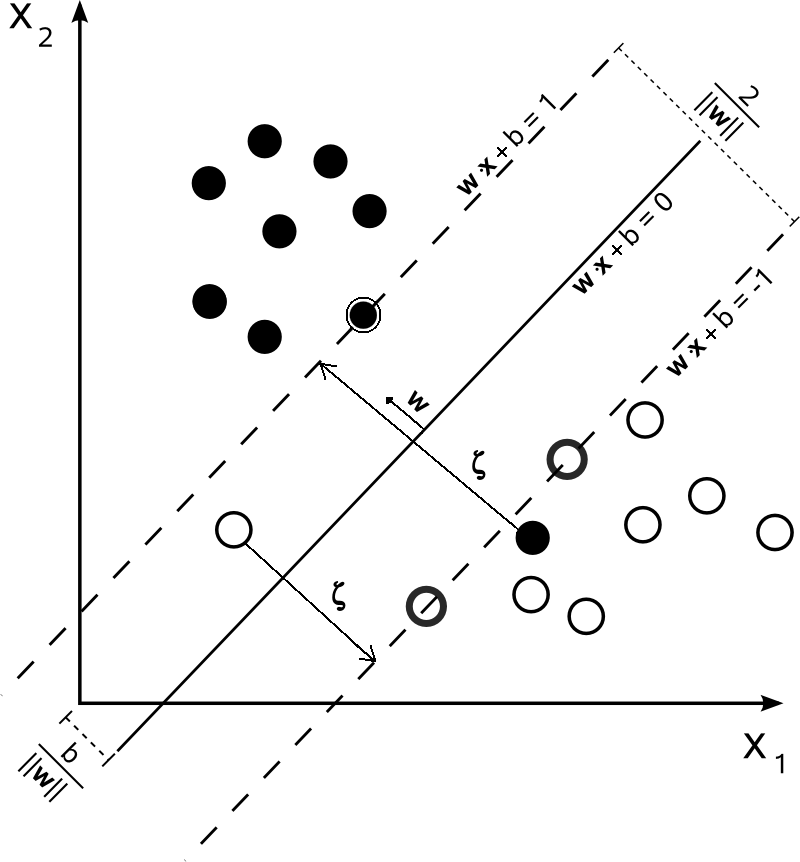
\includegraphics[width=1\linewidth]{./img/svm}
\label{fig:svm}
\end{figure}
\end{column}
\end{columns}
\end{frame}

\begin{frame}
\frametitle{Problema duale}
Il problema in forma duale:
\begin{center}
$\displaystyle\min_{\alpha} \ \frac{1}{2} \ \alpha^{T}Q\alpha - e^{T} \alpha $\newline
subject to $y^{T} \alpha = 0 $ \newline
$ 0 \le \alpha_{i} \le C, \ i = 1,...,l$
\end{center}
La funzione di decisione \`{e} 
\begin{center}
$ sgn( \sum_{i=1}^{N}y_{i}\alpha_{i}K(x_{i},x) + b)$
\end{center}
dove Q  \`{e} una matrice $nxn $ semidefinita positiva, $Q_{ij} \equiv K(x_{i}, x_{j})$ e K \`{e}  la funzione di kernel
\end{frame}

\begin{frame}
\frametitle{Funzione di kernel}
La funzione di kernel pu\`{o} essere una delle seguenti:\newline
\begin{itemize}
\item lineare $ \langle x, x'\rangle $
\item polinomiale $ (\gamma\langle x, x'\rangle + r)^{d} $,
\item rbf $ exp( -\gamma |x, x'|^{2}) $
\item sigmoide $ tanh(\gamma\langle x, x'\rangle + r) $
\end{itemize}
\end{frame}

\subsection{Generazione dei pattern}
\begin{frame}
\frametitle{Generazione dei pattern}
Sono stati generati due diversi input per il modello:
\begin{itemize}
\item Pattern binari
\item PSSM
\end{itemize}
\end{frame}

\begin{frame}
\frametitle{Pattern binari}
\begin{itemize}
\item Pattern sovrapposti di lunghezza fissata N dove ogni amino acido \`{e} rappresentato come un vettore \textit{one hot} lungo 21
\item Pattern corrispondenti ai residui terminali nella catena proteica sono stati generati aggiungendo $(N-1)/2$ \ "dummy" residui X agli estremi della proteina
\item Se il residuo centrale del pattern \`{e} un RNA-interacting residuo, il pattern viene classificato come positivo
\item Viene generato un pattern per ogni residuo della sequenza proteica
\end{itemize}
\end{frame}

\begin{frame}
\frametitle{Pattern binari}
\begin{figure}
\centering
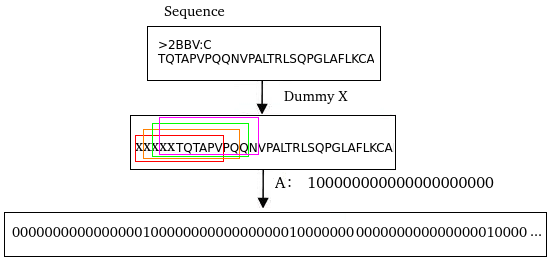
\includegraphics[width=0.7\linewidth]{./img/binary_pattern}
\caption{Generazione pattern binari}
\label{fig:binary_pattern}
\end{figure}
\end{frame}

\begin{frame}
\frametitle{PSSM}
\begin{itemize}
\item L'informazione evoluzionistica ottenuta dall'allineamento multiplo di sequenze fornisce maggiore informazione sulla proteina rispetto all'allineamento singolo
\item Position specific scoring matrix generata da PSI-BLAST contro NCBI nonredundant database
\item Pattern soprapposti ottenuti facendo scorrere una finestra di dimensione $N\ x\ 21 $ sulla matrice
\end{itemize}
\end{frame}

\begin{frame}
\frametitle{PSSM}
\begin{figure}
\centering
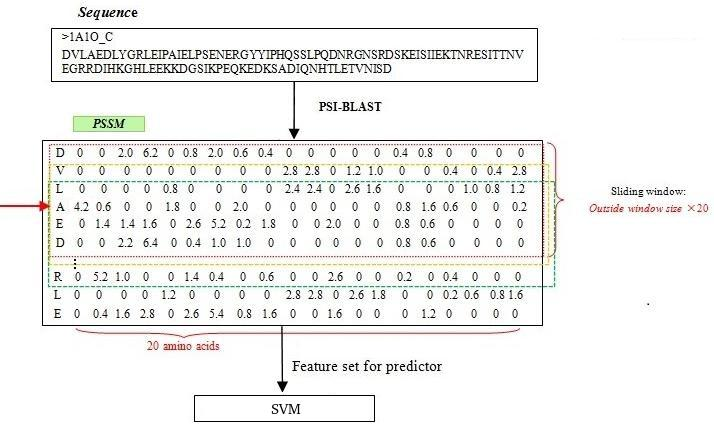
\includegraphics[width=0.7\linewidth]{./img/pssm_pattern}
\caption[]{Generazione feature PSSM}
\label{fig:pssm_pattern}
\end{figure}
\end{frame}

\subsection{Performance}
\begin{frame}
\frametitle{Valutazione delle prestazioni}
\begin{itemize}
\item Per valutare ler performance del modello sono stati calcolati i seguenti parametri:
\begin{itemize}
\item Accuratezza = $\dfrac{TP + TN}{TP + FN + TN + FP}\  X\ 100$
\item Sensitivit\`{a} =  $\dfrac{TP}{TP + FN}\  X\ 100$
\item Specificit\`{a} = $\dfrac{TN}{TN + FP}\  X\ 100$
\item MCC = $\dfrac{TP \ x \ TN - FP \ x \ FN }{\sqrt{(TP+FP)(TP+FN)(TN+FP)(TN+FN)}}\  X\ 100$
\end{itemize}
\item \'{E} stata utilizzata la tecnica del five-fold cross-validation
\end{itemize}
\end{frame}
\end{section}

\begin{section}{Risultati}
\subsection{}
\begin{frame}
\frametitle{Risultati}
\begin{itemize}
\item C = 70
\item $\gamma$ = 0.07
\end{itemize}
\scalebox{0.7}{
\begin{tabular}{lllllll}
\hline \hline
Input Pattern & N & Sensitivity(\%) & Specificity(\%) & Accuracy(\%) & MCC  \\ \hline
		& & & \\	
Binary Pattern & 11 & 33.06 & 90.17 & 76.27 & 0.27 \\
			   & 13 & 31.92 & 92.27 & 77.58 & 0.30 \\
			   & 15 & 30.59 & 93.72 & 78.35 & 0.31 \\
			   & 17 & 29.71 & 94.60 & 78.80 & 0.32 \\
			   & \textbf{19} & \textbf{27.95} & \textbf{95.54} & \textbf{79.08} & \textbf{0.33}\\\hline\hline
		& & & \\	   
PSSM 		   & 11 & 29.27 & 96.56 & 80.18 & 0.37 \\
			   & 13 & 31.92 & 96.50 & 80.78 & 0.40 \\
			   & 15 & 33.33 & 96.19 & 80.88 & 0.40 \\
			   & \textbf{17} & \textbf{34.65} & \textbf{95.88} &\textbf{80.97}  &\textbf{0.41} \\
			   & 19 & 36.06 & 95.28 & 80.86 & 0.40 \\
\hline 
\end{tabular}
}
\end{frame}
\end{section}

\begin{section}{Tecniche semi-supervisionate}
\subsection{Approccio semi-supervisionato}
\begin{frame}
\frametitle{Idea}
\begin{itemize}
\item Partendo dal modello di Kumar si \`{e} cercato di migliorarne l'accuratezza usando come nuove feature rappresentazioni non supervisionate delle sequenze proteiche
\item Tecnica gi\`{a} utilizzata nell'ambito del Natural Language Processing e dell' Handwritten Digit Recognition
\end{itemize}
\end{frame}

\subsection{}
\begin{frame}
\frametitle{Estrazione delle nuove feature}
Utilizzando la libreria \texttt{pylearn2}
\begin{itemize}
\item Implementazione di un Denoising Autoencoder (DAE)
\begin{itemize}
\item Implementazione di una funzione di corruzione dei dati in ingresso all'autoencoder
\item Utilizzo della funzione softmax per aiutare l'autoencoder a ricostruire l'output in modo che rappresenti una sequenza di amino acidi
\end{itemize}
\item Implementazione di una Restricted Boltzmann Machine (RBM)
\end{itemize}
\end{frame}

\subsection{Dataset}
\begin{frame}
\frametitle{RNA\_439}
439 catene proteiche RNA-binding ottenute da quattro diversi dataset
\begin{itemize}
\item Dataset di Kumar (86 catene proteiche)
\item RB198 compilato da Lewis et al. 2010 (198 catene proteiche che condividono meno del 30 \% di similarit\`{a})
\item RB44 costruito da Puton et al. 2012 (44 catene proteiche che condividono meno del 40 \% di similarit\`{a})
\item RB111 composto da 111 catene proteiche che condividono meno del 30 \% di similarit\`{a} e meno del 40 \% con quelle di RB198 e RB44
\end{itemize}
\end{frame}

\subsection{Generazione dei pattern}
\begin{frame}
\frametitle{Generazione dei pattern}
Sono stati generati due diversi input per il modello:
\begin{itemize}
\item Pattern binari di lunghezza N
\item Pattern binari di lunghezza 5, ottenuti con una sliding window dai pattern di lunghezza N
\end{itemize}
\end{frame}
\end{section}

\begin{section}{Denoising Autoencoders}
\begin{frame}
\frametitle{Denoising Autoencoders}
\begin{itemize}
\item Estensione di un classico autoencoder
\item L'autoencoder viene allenato a riscostruire l'input a partire da una versione corrotta di questo, per forzare i livelli nascosti a scoprire feature pi\`{u} robuste
\item Il processo di corruzione \`{e} di tipo stocastico
\begin{itemize}
\item Corruttore gaussiano: aggiunge rumore gaussiano con media nulla all'input 
\item Corrutore one-hot: cambia l'elemento attivo con una certa probabilit\`{a}
\end{itemize}
\end{itemize}
\end{frame}

\subsection{Denoising Autoencoder}
\begin{frame}
\frametitle{Definizione}
\begin{figure}
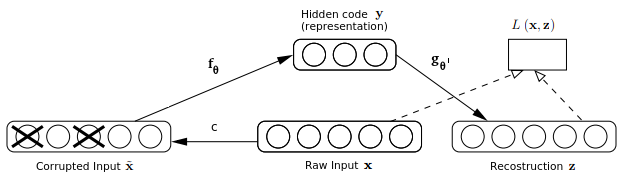
\includegraphics[width=0.7\linewidth]{./img/dae}
\label{fig:dae}
\end{figure}
\begin{itemize}
\item L'input corretto $ \boldsymbol{x} \in [0,1]^{d}  $ viene parzialmente corrotto,$ \boldsymbol{\widetilde{x}} $
\item $ \boldsymbol{\widetilde{x}} $ viene mappato in una rappresentazione nascosta $ \boldsymbol{y} = sigmoid(\boldsymbol{W\widetilde{x}+ b}) $
\item A partire da y viene ricostruito $ \boldsymbol{z} = sigmoid(\boldsymbol{W'y+ b'})$
\item Il modello viene trainato in modo che i parametri minimizzino l'errore di ricostruzione $ \textbf{L(x,z)} = || x - z ||^{2} $
\end{itemize}
\end{frame}
\end{section}

\begin{section}{Risultati}
\subsection{Approccio semi-supervisionato con DAE}
\begin{frame}
\frametitle{Risultati}
\begin{itemize}
\item \#unit\`{a} nascoste = 500
\item \#epoche = 100
\end{itemize}
\scalebox{0.85}{
\begin{tabular}{llllll}
\hline \hline
Input Pattern & N & Sensitivity(\%) & Specificity(\%) & Accuracy(\%) & MCC  \\ \hline
	& & & & &\\	
Binary Pattern & \textbf{5} & \textbf{28.13} & \textbf{93.21} 
						& \textbf{77.36} & \textbf{0.28} \\
			   & 11 & 30.68 & 89.49 & 75.17 & 0.23 \\   
\hline 
\end{tabular}
}
\end{frame}
\end{section}


\begin{section}{RBM}
\subsection{Restricted Boltzmann Machine}
\begin{frame}
\frametitle{Definizione}
\begin{columns}
\begin{column}{6cm}
\begin{itemize}
\item Markov Random Field associate con un grafo non orientato bipartito
\item Valori binari per unit\`{a} visibili e unit\`{a} nascoste
\end{itemize}
\end{column}
\begin{column}{4cm}
\begin{figure}
\centering
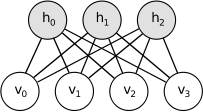
\includegraphics[width=1\linewidth]{./img/rbm}
\label{fig:rbm}
\end{figure}
\end{column}
\end{columns}
\begin{itemize}
\item La probabilit\`{a} congiunta \`{e} data dalla distribuzione di Gibbs:
\begin{center}
$ p(v,h) = \frac{1}{Z}e^{-E(v,h)} $\newline
$ Z = \sum_{v} \sum_{h}e^{E(v,h)} $ \newline
$ E(v,h) = -\sum_{i=1}^{n}\sum_{j=1}^{m}w_{ij}h_{i}v_{j} -\sum_{j=1}^{m}b_{j}v_{j} - \sum_{i=1}^{n}c_{i}h_{i} $
\end{center}
\end{itemize}
\end{frame}

\begin{frame}
\frametitle{Training}
\begin{itemize}
\item  $ \ \ \ \  \ \ \ \ \ \ \ \ \ \ \ \ \ \ \ \ \ \ \ \displaystyle\max_{w,b,c} \ \log p(v)$ 
\begin{center}
$p(v) =\frac{1}{Z} \sum_{h}p(v,h) =\frac{1}{Z} e^{-F(v)}$
$F(v) = -log\sum_{h}e^{-E(v,h)} -\sum_{j=1}^{m}b_{j}v_{j} $\newline
\end{center}
\end{itemize}
\begin{columns}
\begin{column}{6cm}
\begin{itemize}
\item Contrastive Divergence
\end{itemize}
\end{column}
\begin{column}{4cm}
\begin{figure}
\centering
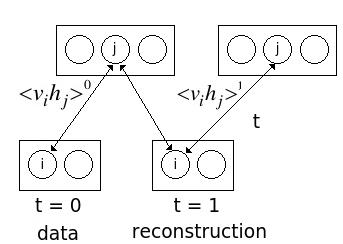
\includegraphics[width=1\linewidth]{./img/cd}
\label{fig:cd}
\end{figure}
\end{column}
\end{columns}
\end{frame}
\end{section}

\begin{section}{Risultati}
\subsection{Approccio semi-supervisionato RBM}
\begin{frame}
\frametitle{Risultati}
\begin{itemize}
\item \#unit\`{a} nascoste = 500
\item \#epoche = 100
\end{itemize}
\scalebox{0.85}{
\begin{tabular}{llllll}
\hline \hline
Input Pattern & N & Sensitivity(\%) & Specificity(\%) & Accuracy(\%) & MCC  \\ \hline
	& & & & &\\	
Binary Pattern  & 5 & 9.2  & 98.92 & 78.73 & 0.20 \\ 
				& \textbf{11} & \textbf{22.32} & \textbf{96.99} 
						& \textbf{80.19} & \textbf{0.30} \\
			     
\hline 
\end{tabular}
}
\end{frame}
\end{section}

\begin{section}{Confronto}
\subsection{}
\begin{frame}
\frametitle{Confronto}
\scalebox{0.7}{
\begin{tabular}{lllllll}
\hline \hline
Metodo & Input Pattern & N & Sensitivity(\%) & Specificity(\%) & Accuracy(\%) & MCC  \\ \hline
	& & & & &\\	
SVM & Binary Pattern  & \textbf{17} & \textbf{29.71} & \textbf{94.60} & \textbf{78.80} & \textbf{0.32} \\
							& & & & & &\\	  
& PSSM 		    & \textbf{17} & \textbf{34.65} & \textbf{95.88} &\textbf{80.97}  &\textbf{0.41} \\
 \hline\hline   
									  
							& & & & & &\\	
DAE + SVM & Binary Pattern & \textbf{5} & \textbf{28.13} & \textbf{93.21} 
						& \textbf{77.36} & \textbf{0.28} \\ \hline\hline
									  
							& & & & & &\\	
RBM + SVM& Binary Pattern & \textbf{11} & \textbf{22.32} & \textbf{96.99} 
						& \textbf{80.19} & \textbf{0.30} \\

\hline 
\end{tabular}
}
\end{frame}
\end{section}
\end{document}
